On procède à l'insertion: \newline
    \begin{tt} > mongoimport -type -json -d geodb -c earthquakes --file
eartquakes.json \end{tt} \newline
    Puis on applique les modifications :
\begin{lstlisting}[language=Mongo, caption=]
db.earthquakes.find().forEach(
    function(eq){
        eq.properties.iso_date = new Date(eq.properties.time);
        db.earthquakes.save(eq);
    }
);
\end{lstlisting}

    Le sujet propose de convertir la chaîne de caractère du champ properties.types en tableau et le mettre dans un champ types\_as\_array.
    
    \begin{lstlisting}[language=Mongo, caption=Chaine de carractères vers tableau.]
    db.earthquakes.find().forEach( function(eq){
        eq.properties.types_as_array= eq.properties.types.split(",");
        eq.properties.types_as_array.shift();
        eq.properties.types_as_array.pop();
        db.earthquakes.save(eq);
        } 
    );
    \end{lstlisting}
    \begin{block}{Reamrque}
        Si on observe un ou deux documents au hasard on remarque que tous les champs types commencent et finissent par un séparateur. Une case vide se créer au début et à la fin du tableau, c’est assez dommage. De mémoire il existe <array>.shift() en javascript. Impossible de retrouver cette fonction dans la doc mongodb, on l’essai donc directement sur l’attribut du document aux lignes 3 et 4. 
    \end{block}

    \par
    Comme en JavaScript, la méthode ne retourne pas un tableau mais affecte directement le tableau en question et donc, ici, le document. On affiche un document pour  tester la requête.
    
    \begin{lstlisting}[language=Mongo, caption=Accès aux tableau Types\_as\_array d"un document.]
db.earthquakes.findOne({},
    {
        id:1,
        "properties.types":1,
        "properties.types_as_array":1
    }
);
    \end{lstlisting}
    
    \begin{lstlisting}[language=JSON, caption=Tableau de types et la chaine de carractère.]
    :/* 0 */
{
    "_id" : ObjectId("54a038b2237aba92e1072616"),
    "properties" : {
        "types" : ",general-link,geoserve,nearby-cities,origin,phase-data,scitech-link,",
        "types_as_array" : [ 
            "general-link", 
            "geoserve", 
            "nearby-cities", 
            "origin", 
            "phase-data", 
            "scitech-link"
        ]
    },
    "id" : "nc72001620"
}
    \end{lstlisting}
    
La question suivante conserne le nettoyage des données.\newline
Ah zut … Avec la remarque précédente on a grillé les étapes :(.
On l’a fait quand même? \newline
Après avoir rechargé la base de données, on confirme le bon fonctionnement de la requête suivante.
\begin{lstlisting}[language=Mongo, caption=Nettoyage des données.]
db.earthquakes.update( 
    {},
    { $pullAll: { "properties.types_as_array": [""] } },
    { multi: true }
);
\end{lstlisting}

\subsection{requêtage}
    \begin{itemize}
    \item Donnez le nombre de documents dont la liste de type contient "geoserves" et "tectonic-summary » 
       \begin{lstlisting}[language=Mongo, caption=]
    db.earthquakes.find({
        "properties.types_as_array":{$all:["geoserve",
        "tectonic-summary"]
        }
    }).count()
\end{lstlisting}

le résultat retourné est 2954
\begin{block}{Remarque} L’énoncé indique entre crochet «geoserves» avec un S, ce qui donne zéro résultats. Attention aux copier/coller.
\end{block}


    \item Ecrire une requête qui donne le nombre de tremblements de terre en Californie (Indice : RegExp) 
       \begin{lstlisting}[language=Mongo, caption=]
    db.earthquakes.find({
        "properties.place": { $regex: /California$/, $options: "i"} 
    }).count()

\end{lstlisting}
Explication: on remarque que le l’état est placée à la fin du champ properties.place. La requête précédente compte tous les document dont le champ properties.place termine par California (Sans prendre en compte les Majuscules).\newline
le résultat retourné est 3535.
\end{itemize}

\subsection{Coordonnées et dimensions}
Pour cette question on proprose un code directement tapé dans l'interface RoboMongo. On rapelle que ce code peut être écrit dans un fichier JavaScript et passé en console par la commande mongo.

\begin{lstlisting}[language=Javascript, caption=Création du champ "depth".]
var nbDocs = db.earthquakes.find().count()
var nbComplying = db.earthquakes.find({"geometry.coordinates":{$size :3}}).count()
if (nbComplying ==  nbDocs) { // si tous les docs respectent le meme schema
    allDocs = db.earthquakes.find()
    var j = 0
    for (var i = 0; i < nbDocs; i++) { 
        var value = allDocs[i].geometry.coordinates[2]; // recuperation de la valeur
        allDocs[i].depth = value; // creation du champ depth
        j = j+1;
        db.earthquakes.save(allDocs[i]); //svgarde du doc courant
    }
    print(j +" Documents ont ete modifies et inseres.");

    db.earthquakes.update({},{$pop: {"geometry.coordinates": 1}}, {multi: true});
}
\end{lstlisting}

\begin{block}{Explication} Avant de supprimer le dernier élément de chaque tableau, "geometry.coordinates" on vérifie qu'ils aient tous les 3 éléments (l.4). Puis on boucle sur tous les éléments présents en leur ajoutant le champ depth. (l.9). Une fois tous les documents édités on modifie directement la collection en suppriment le dernier élément du tableau "coordinates" (l.15).
\end{block}

Le code retourne l'inscription : 7669 Documents ont été modifiés et insérés. \newline 

Pour vérifier le bon déroulement du script on passe la commande suivante: 

\begin{figure}[h!]

    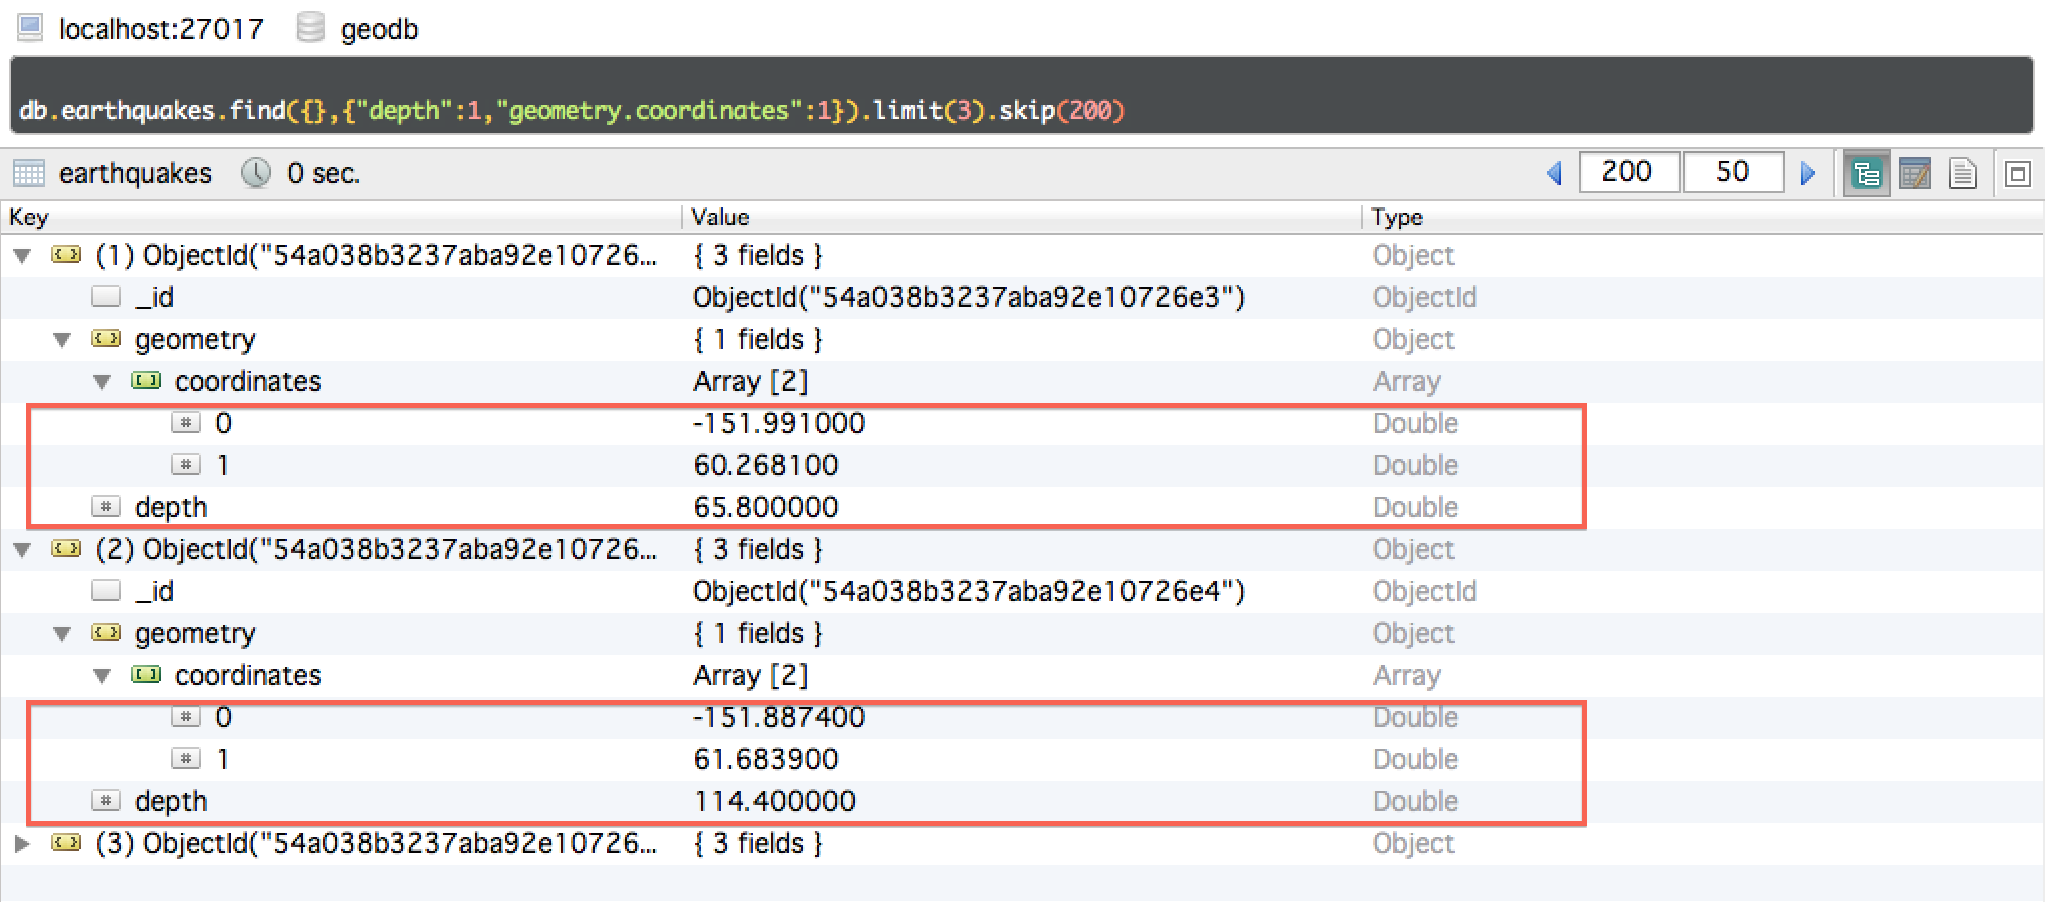
\includegraphics[scale=0.4]{img/depth.png}
    \caption{...find({},{"depth": 1, "geometry.coordinates": 1}).limit(3).skip(200)}
    \end{figure}

\subsection{Indexation géographique}
    MongoDB propose plusieurs types d'index, dont les "géospacial Indexes". Ils permettent de gérer des informations sur plusieurs dimensions (coordonnées, distance, position...). Il y en a notament un index pour les coordonées cartésienne et un autre pour les sphériques. L'index demandé est de type 2d.
    
    \par Ce type d'index prend en charge les coordonnées plannes  et ne supporte pas l'utilisation d"objet GeoJSON (contrairement à 2dsphere). Il prend comme argument le champ support de l'index et les options min, max bits. Par défaut mongodb considère les valeurs commes des longitudes et latitudes, elles vont donc de -190 à 190. Si une valeur sort de se cette fourchette mongodb renvoie un erreur. 
    
    \par Avant de créer l'index on vérifie donc que le jeux de données respecte bien cette convention avec les reqêtes suivantes : \newline
    \begin{tt} db.earthquakes.find({"geometry.coordinates": {\$gt: 10}}).count() \end{tt} \newline 
    \begin{tt} db.earthquakes.find({"geometry.coordinates": {\$lt: 10}}).count() \end{tt} \newline
    
    Le résultat est zero, les données sont adaptées, on ne préscise donc pas d"option.
    \begin{lstlisting}[language=Mongo, caption=]    
    db.earthquakes.ensureIndex({"geometry.coordinates": "2dsphere"})
    \end{lstlisting}
    
\newpage

    On peut alors requêter sur ce champs en utilisant des fonctions géométriques proposées par mongodb comme: \$geoIntersects, \$geoWithin, \$near. Exemple, exécuter une requête qui cherche les tremblements de terre
proche de la position -3.984,48.724 

    \begin{lstlisting}[language=Mongo, caption=]    
    db.earthquakes.find({
        "geometry.coordinates":
        {
            $near : [-3.984, 48.724],
            $maxDistance: 1000
        }
    });
    \end{lstlisting}